\documentclass[a4paper,12pt]{article}
\usepackage{amssymb}
\usepackage{amsfonts}
\usepackage{amsthm}
\usepackage{amsmath}
\usepackage[T1]{fontenc}
\usepackage[utf8]{inputenc}
\usepackage[british]{babel}
\usepackage{times}
\usepackage{anysize}
\usepackage{color}
\usepackage{listings}
\usepackage{graphicx}
\usepackage{enumerate}
\usepackage{multicol}
\usepackage{float}

\usepackage{lmodern}  % for bold teletype font
\usepackage{xcolor}   % for \textcolor
%\lstloadlanguages{matlab}
\lstset{
	basicstyle=\ttfamily,
	columns=fullflexible,
%	frame=single,
	breaklines=true,
	postbreak=\mbox{\textcolor{red}{$\hookrightarrow$}\space},
}

\begin{document}
\begin{titlepage}
\center
\vspace*{\fill}
\Huge{Modeling of Physical Systems}\\
\Large{Application of box models to Upper
Danube catchment simulation.}\\
\vspace*{1.5cm}
Dominik Katszer\\
\large{28 April 2018}
\vspace*{1.5cm}
\vspace*{\fill}
\end{titlepage}
\section{Aim of laboratory}
The aim of the laboratory is to calculate a mean residence time of water in the  Danuba river using modelled object called "black-box". This river was choosen because of accessibility to data accross many years. According to it, it is possible to connect water amount
increasing with any occurrence.
\section{Algorithm}
In order to obtain information about river characteristics we are basing on tracer experiment. Basing on that experiment, it is possible to calculate any other response of the system. In this case , in order to calculate  river catchments I used exponential model.
\begin{equation}
	C(t) = \int_{- \infty}^{t} C_{in}(t') \cdot g(t - t') \cdot e^{-\lambda \cdot (t - t')} dt'
\end{equation}
Where:
\begin{itemize}
    \item t - time variable
	\item $C(t)$ - output function
    \item $C_{in}(t')$ - input function
    \item $g(t - t') = t_t^{-1}*e^{\frac{-(t-t')}{t_t}}$ - exponential model
    \item $t_t$ - mean residence time
    \item $\lambda = 4.696 * 10^{-3}$ - radioactive decay constant
\end{itemize}

\section{Results}
By changing mean residence time $t_t$ I tried to change the result of the simulation in order to be as similar to real data as possible. At the beggining manuall method was used and results are presented in the figure below.
\begin{figure}[H]
\centerline{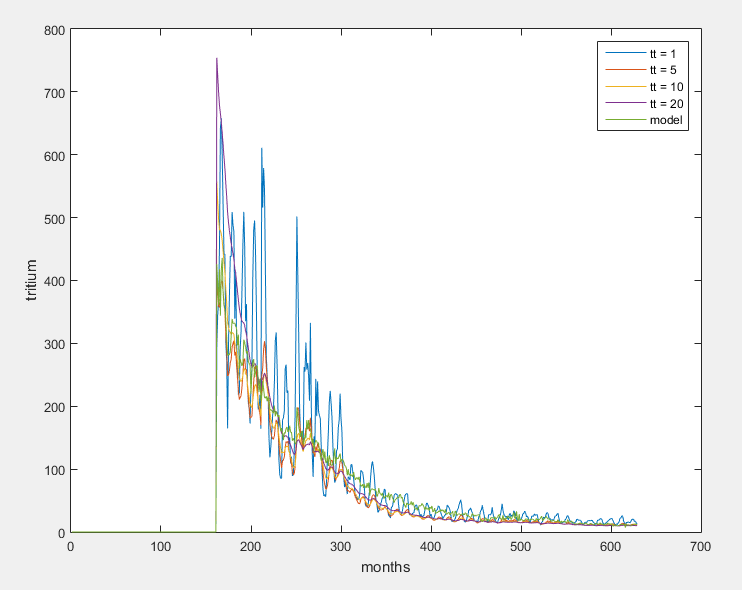
\includegraphics[scale=0.8]{manuall}}
\end{figure}
After that automatic strategy was applying which calculates value of $t_t$ basing on the difference between original data and calculated result. 
\begin{figure}[H]
\centerline{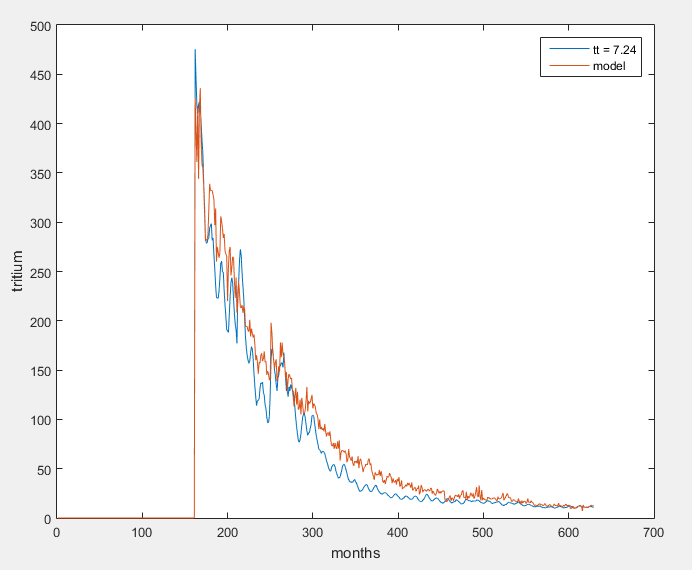
\includegraphics[scale=0.8]{calculated}}
\end{figure}

\section{Conclusions}
This report covered simplified methods to calculate the mean residence time of water in the upper part of the Danube river using black box modeling with exponential transit function. This kind of exercise is difficult to make
because it needs long term measurement to validate precision of calculation. 
\section{Source code}
\textbf{main.m}\\
\lstinputlisting{main.m}
\textbf{blackBox.m}\\
\lstinputlisting{blackBox.m}
\textbf{expoModel.m}\\
\lstinputlisting{expoModel.m}
\textbf{forward.m}\\
\lstinputlisting{forward.m}

\end{document}